\chapter{Phân tích PIDNet}
\section{Từ mạng hai nhánh đến vấn đề overshoot}
Trong mạng encoder--decoder, encoder giảm kích thước feature map để mỗi vị trí nhìn được một vùng ảnh rộng hơn. Vùng ảnh đó được gọi là receptive field. Nhờ có ngữ cảnh rộng, mạng dễ nhận ra một vùng là mặt đường hay tòa nhà, nhưng có thể làm mất chi tiết của cột mảnh hoặc người ở xa. Upsampling chỉ tăng kích thước feature map; những chi tiết đã mất vẫn cần được bổ sung từ các tầng có độ phân giải cao. Dilated convolution và mạng nhiều độ phân giải là hai cách giữ thêm chi tiết, với chi phí tính toán khác nhau.

BiSeNet \cite{bisenet} giải quyết bài toán bằng hai luồng: một luồng giữ chi tiết, một luồng học ngữ cảnh. DDRNet \cite{ddrnet} cũng duy trì hai độ phân giải và cho hai luồng trao đổi thông tin nhiều lần. Khi ghép chúng bằng fusion, ngữ cảnh vẫn có thể lấn át chi tiết ở biên. Chẳng hạn, một cột nhỏ nằm giữa vùng đường và tòa nhà có thể bị gán thành nền vì phần lớn receptive field chứa pixel nền, dù luồng chi tiết còn nhận ra đường viền cột.

Bài báo gọi sự lan nhãn qua biên này là \emph{overshoot}, lấy ý tưởng từ đáp ứng vượt mức trong điều khiển. Vấn đề cần xử lý là quyết định nơi nào nên dựa nhiều vào ngữ cảnh, nơi nào cần giữ chi tiết. PIDNet bổ sung nhánh D để học vị trí biên, rồi dùng thông tin đó khi ghép hai luồng còn lại.

\section{Cơ sở PID và ý nghĩa của nhánh D}
\subsection{PID truyền thống}
Với sai số $e(t)=r(t)-y(t)$ giữa giá trị đặt và đầu ra hệ thống, dạng PID liên tục lý tưởng là
\begin{equation}
 u(t)=K_Pe(t)+K_I\int_0^t e(\tau)\,d\tau+K_D\frac{de(t)}{dt}.
 \label{eq:pid-continuous}
\end{equation}
Trong công thức trên, $u(t)$ là tín hiệu điều khiển; $K_P$, $K_I$ và $K_D$ là hệ số của ba thành phần. P phản ứng với sai số hiện tại, I cộng dồn sai số theo thời gian, còn D phản ứng với tốc độ thay đổi của sai số. Khi lấy mẫu theo từng bước và gộp chu kỳ lấy mẫu vào các hệ số, công thức trở thành
\begin{equation}
 u[n]=k_pe[n]+k_i\sum_{j=0}^{n}e[j]
      +k_d\big(e[n]-e[n-1]\big).
 \label{eq:pid-discrete}
\end{equation}
Ở đây, $n$ là bước thời gian và $k_p,k_i,k_d$ là các hệ số rời rạc. Khi sai số đang giảm, hiệu $e[n]-e[n-1]$ có thể âm. Hạng D khi đó bù bớt tác dụng của hạng I đang còn tích lũy nhiều sai số, giúp giảm overshoot. Công thức (1) của bài báo trình bày hai hạng P và I; Hình~3 bổ sung vai trò của D như trong biểu thức~\eqref{eq:pid-discrete}.

Có thể nhìn ba thành phần này dưới góc độ lọc tín hiệu. Với điều kiện đầu bằng 0, hàm truyền trong miền $z$ và đáp ứng theo tần số là
\begin{align}
 C(z)&=k_p+\frac{k_i}{1-z^{-1}}+k_d(1-z^{-1}),\label{eq:pid-z}\\
 C(e^{j\omega})&=k_p+\frac{k_i}{1-e^{-j\omega}}
                     +k_d(1-e^{-j\omega}).\label{eq:pid-frequency}
\end{align}
Trong đó, $z$ là biến của phép biến đổi Z; thay $z=e^{j\omega}$ cho đáp ứng tại tần số góc $\omega$, với $j^2=-1$. Biểu thức~\eqref{eq:pid-frequency} tương ứng công thức (4) của bài báo. Độ lớn đáp ứng của riêng I và D, bỏ qua hệ số khuếch đại, là
\begin{equation}
 |H_I(e^{j\omega})|=\frac{1}{2|\sin(\omega/2)|},\qquad
 |H_D(e^{j\omega})|=2|\sin(\omega/2)|.
 \label{eq:pid-magnitudes}
\end{equation}
Với $0<\omega\leq\pi$, I có độ khuếch đại lớn ở tần số thấp, còn D nhấn mạnh tần số cao; P giữ độ khuếch đại không đổi. Trên ảnh, vùng mặt đường có màu và nhãn thay đổi chậm là ví dụ về thành phần tần số thấp. Mép giữa người đi bộ và nền thay đổi nhanh hơn, nên chứa nhiều thành phần tần số cao. Tác giả dựa vào đặc điểm này để gắn I với ngữ cảnh và D với biên. Tần số ở đây mô tả sự thay đổi theo vị trí trong ảnh.

\begin{figure}[htbp]
\centering
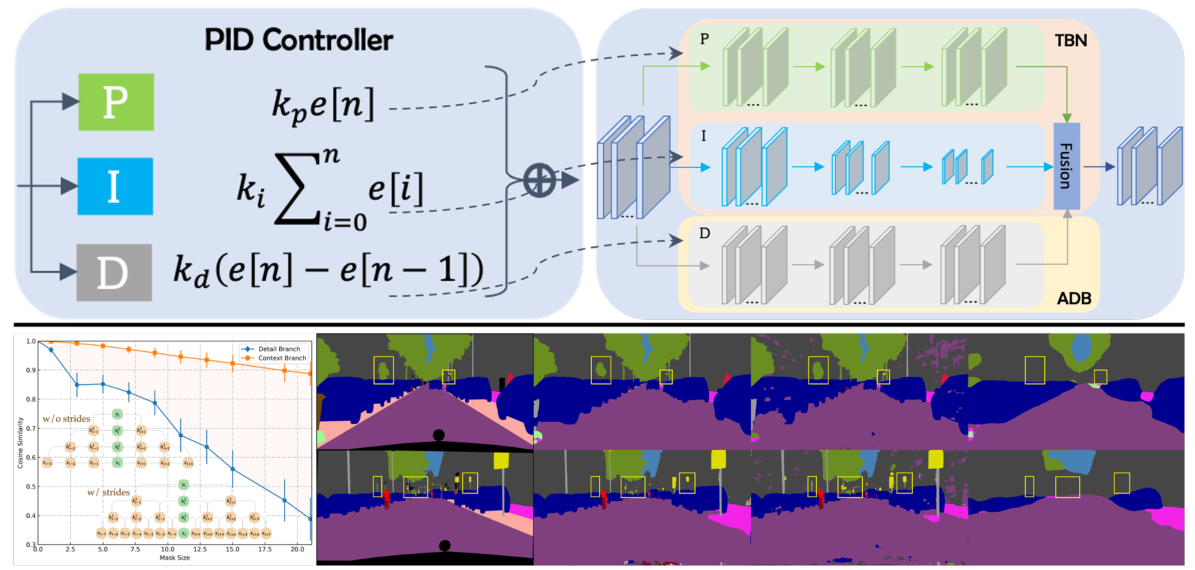
\includegraphics[width=.85\linewidth]{assets/pidnet/pid-analogy.png}
\caption{Phép tương tự giữa PID và mạng ba nhánh; phần dưới minh họa độ nhạy với ngữ cảnh và dự đoán của từng luồng DDRNet. Trích Hình~3 của Xu và cộng sự, CVPR 2023 \cite{pidnet}.}
\label{fig:paper-pid-analogy}
\end{figure}

\subsection{Từ phép tương tự PID đến CNN}
Để giải thích sự khác nhau giữa detail và context, bài báo xét hai CNN một chiều gồm ba tầng và bỏ BatchNorm, ReLU để phép tính dễ theo dõi. Các công thức (2)--(3) được viết gọn như sau:
\begin{align}
 O_{\mathrm{detail}}[i]&=\sum_{r=-3}^{3}K^D_{i+r}x[i+r],\label{eq:toy-detail}\\
 O_{\mathrm{context}}[i]&=\sum_{r=-7}^{7}K^C_{i+r}x[i+r].\label{eq:toy-context}
\end{align}
Ở đây, $x[i+r]$ là giá trị đầu vào cách vị trí $i$ một khoảng $r$; các hệ số $K$ được tạo từ trọng số convolution của ba tầng. Luồng detail chỉ dùng bảy vị trí từ $i-3$ đến $i+3$, còn context dùng 15 vị trí từ $i-7$ đến $i+7$. Context vì vậy tổng hợp thông tin trên vùng rộng hơn, tương tự vai trò cộng dồn của I; detail giữ thay đổi cục bộ tốt hơn, gần với P. Chữ $D$ trong $K^D$ viết tắt cho \emph{detail}, khác với tên nhánh D của PIDNet.

Phép tương tự này là cơ sở thiết kế mạng. CNN thực tế còn có trọng số học được, BatchNorm, ReLU và residual connection, nên đáp ứng phức tạp hơn các bộ lọc trên. PIDNet dùng ba nhánh để học chi tiết, ngữ cảnh và biên trong ảnh; mạng không tích lũy sai số theo thời gian như một bộ điều khiển PID.

\section{Kiến trúc ba nhánh và trao đổi thông tin}
\subsection{Residual block và luồng đặc trưng trong PIDNet-S}
PIDNet-S được ghép từ các residual block \cite{pidnet,pidnetcode}. BasicBlock dùng hai convolution $3\times3$. Bottleneck dùng chuỗi $1\times1$, $3\times3$, $1\times1$, với số kênh đầu ra gấp đôi số kênh bên trong. Trong mỗi block, shortcut đưa đầu vào đến phép cộng với kết quả của nhánh convolution. Mạng nhờ đó học phần thay đổi cần thêm vào đặc trưng đã có. Với block có ReLU sau phép cộng,
\begin{equation}
 \mathbf h_{k+1}=\operatorname{ReLU}\!\left(F_k(\mathbf h_k)+S_k(\mathbf h_k)\right).
 \label{eq:residual-block}
\end{equation}
Trong đó, $\mathbf h_k$ là đầu vào block thứ $k$, $F_k$ là nhánh convolution, còn $S_k$ là shortcut. Khi kích thước không đổi, $S_k(\mathbf h_k)=\mathbf h_k$. Khi đổi số kênh hoặc stride, shortcut dùng convolution $1\times1$ và BatchNorm để hai vế có cùng kích thước trước khi cộng. Một số block bỏ ReLU sau phép cộng.

Hai convolution đầu và hai tầng residual tạo đặc trưng dùng chung, rồi mạng tách thành P, I và D như Bảng~\ref{tab:pidnet-s-feature-flow}. Các block tiếp theo xử lý đặc trưng trong từng nhánh; Pag và các kết nối I--D giúp chúng trao đổi thông tin. Trước Light-Bag, P và D đều có 128 kênh trên lưới bằng $1/8$ ảnh đầu vào. PAPPM đưa I về 128 kênh, rồi upsampling đến cùng lưới để fusion. Đầu ngữ nghĩa sau đó xuất 11 logit tại mỗi vị trí và nội suy về kích thước ảnh CamVid.

\begin{table}[htbp]
\centering\small
\begin{tabularx}{\linewidth}{@{}lXcc@{}}
\toprule
Luồng & Các tầng chính & Tỷ lệ không gian & Số kênh\\
\midrule
Dùng chung & Hai convolution $3\times3$; hai BasicBlock & $1/4$ & 32\\
Dùng chung & Hai BasicBlock, block đầu stride 2 & $1/8$ & 64\\
P & Hai tầng, mỗi tầng hai BasicBlock; một Bottleneck & $1/8$ & 128\\
I & Hai tầng, mỗi tầng ba BasicBlock; hai Bottleneck & $1/16\to1/32\to1/64$ & $128\to256\to512$\\
I & PAPPM và upsampling & $1/8$ & 128\\
D & Một BasicBlock; hai Bottleneck & $1/8$ & $32\to64\to128$\\
Fusion & Light-Bag & $1/8$ & 128\\
Đầu ra & Đầu ngữ nghĩa; nội suy về ảnh gốc & $1/8\to1$ & 11\\
\bottomrule
\end{tabularx}
\caption{Luồng đặc trưng của PIDNet-S với $C=32$, $m=2$, $n=3$ và đầu phân đoạn 11 lớp. Tỷ lệ không gian là mức giảm danh nghĩa so với ảnh đầu vào; kích thước các tầng sâu còn phụ thuộc padding và làm tròn. Các kết nối Pag và I--D được minh họa ở Hình~\ref{fig:paper-architecture}.}
\label{tab:pidnet-s-feature-flow}
\end{table}

\begin{figure}[htbp]
\centering
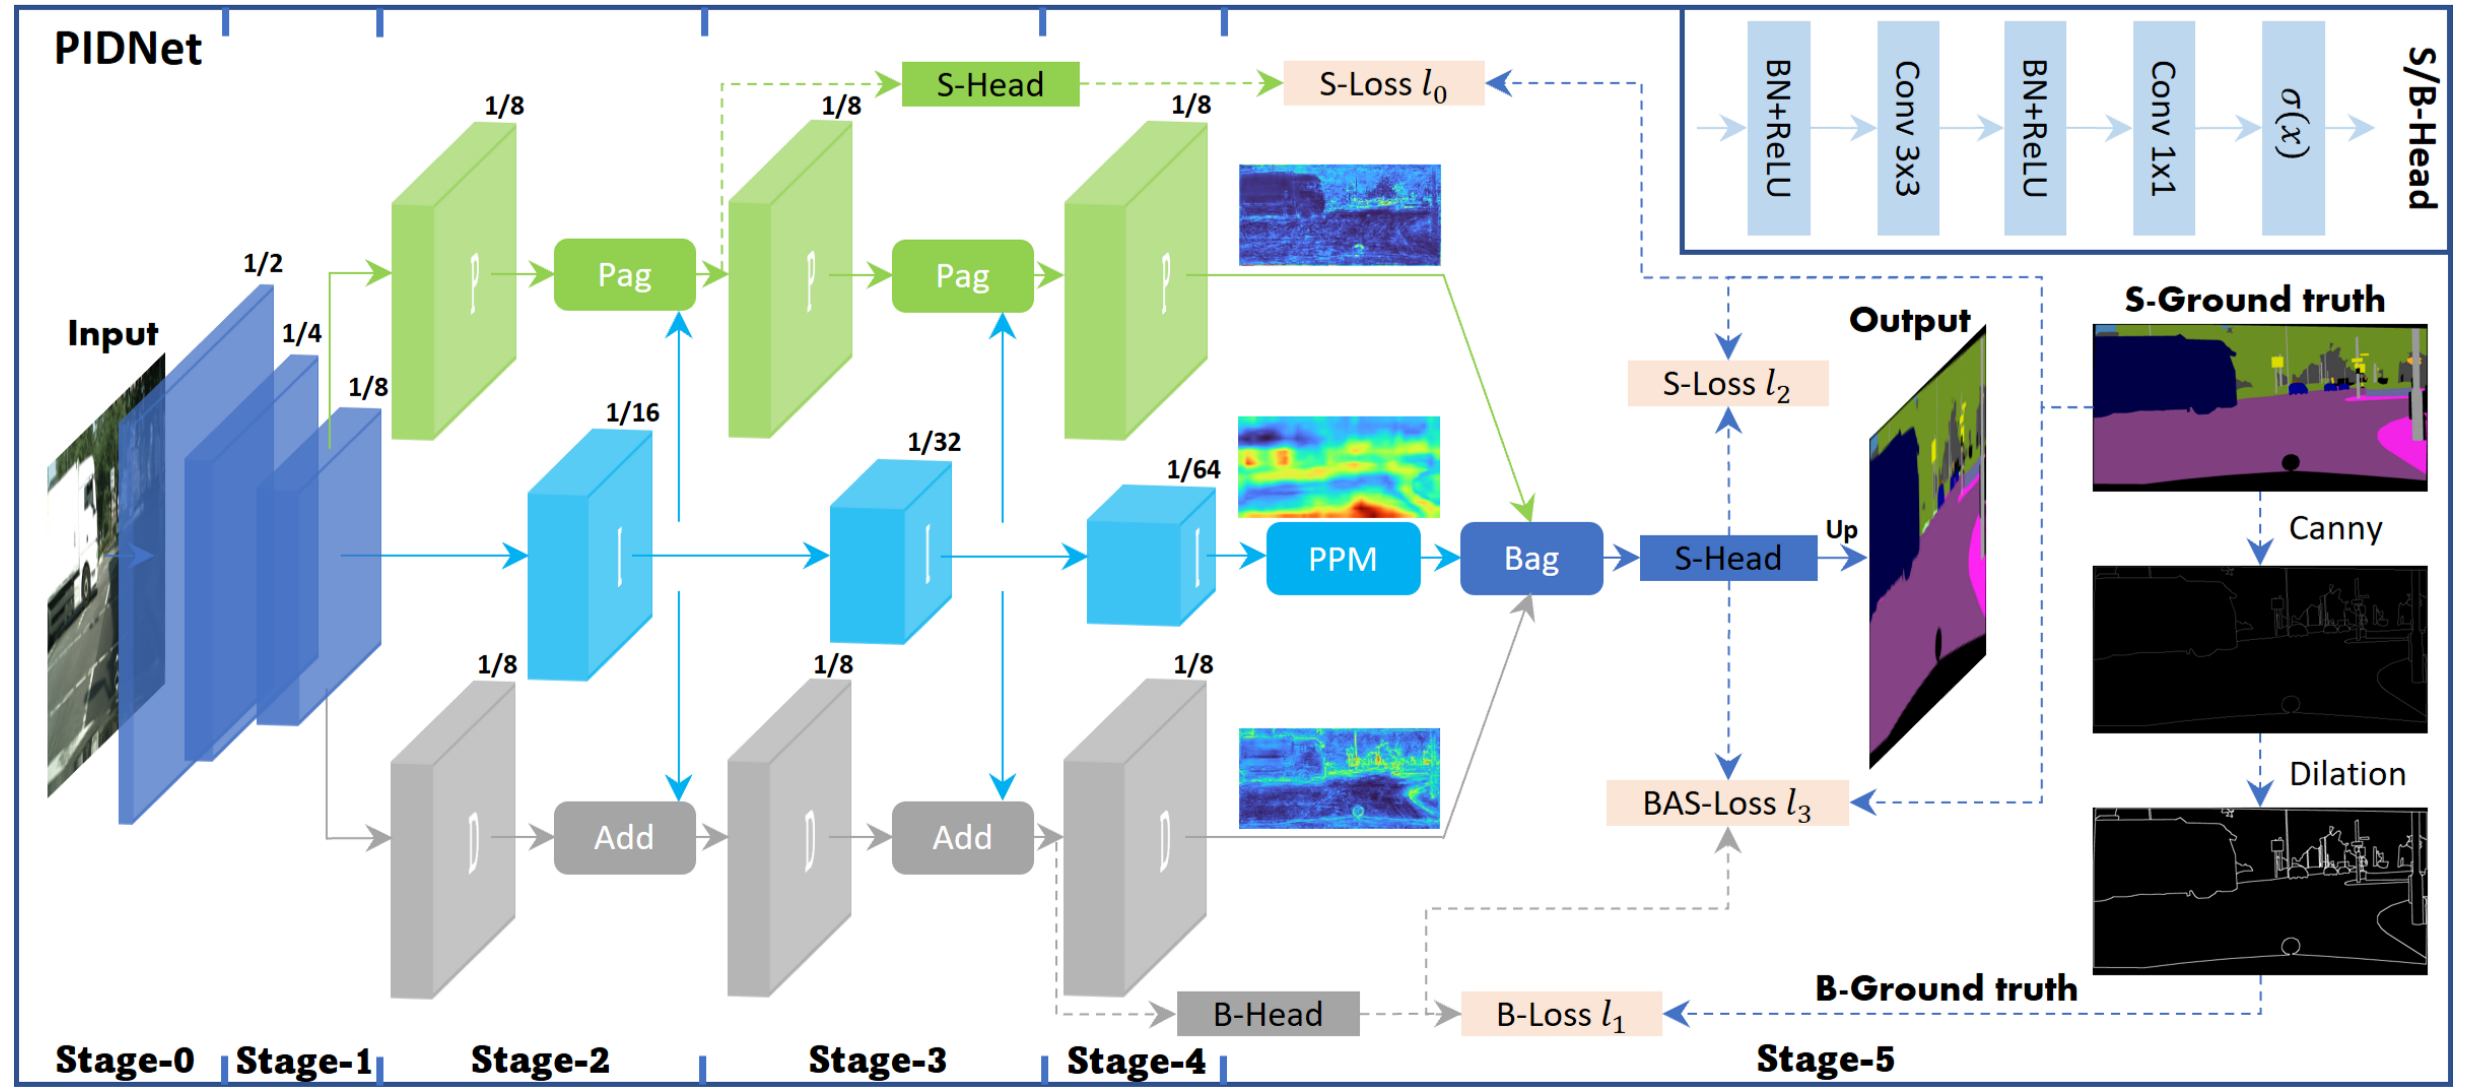
\includegraphics[width=\linewidth]{assets/pidnet/architecture.png}
\caption{Kiến trúc PIDNet. P giữ feature map độ phân giải cao; I tổng hợp ngữ cảnh; D học thông tin biên. S-Head và B-Head là các đầu ngữ nghĩa và biên. Các đường nét đứt phục vụ loss khi train. Trích Hình~4 của Xu và cộng sự \cite{pidnet}.}
\label{fig:paper-architecture}
\end{figure}

Hình~\ref{fig:paper-architecture} cho thấy cách ba nhánh chia việc:
\begin{itemize}
 \item \textbf{P (proportional):} giữ feature map ở khoảng $1/8$ kích thước ảnh. Nhánh này theo dõi vị trí và đường viền, chẳng hạn hình dạng người đi bộ hay cột bên đường. Số tầng vừa phải giúp giảm chi phí tính toán trên lưới lớn.
 \item \textbf{I (integral):} giảm dần độ phân giải qua các mức $1/16$, $1/32$ và $1/64$. Nhánh này dùng nhiều tầng hơn để nhận ra lớp từ ngữ cảnh rộng, chẳng hạn phân biệt mặt đường với vỉa hè.
 \item \textbf{D (derivative):} học vị trí chuyển từ lớp này sang lớp khác. Nhãn biên tạo từ mặt nạ phân đoạn giúp D tập trung vào đường phân cách ngữ nghĩa.
\end{itemize}
I gửi ngữ cảnh sang P qua Pag và sang D qua phép cộng. Ví dụ, một cạnh mạnh có thể là mép ô tô hoặc chỉ là bóng đổ trên đường; ngữ cảnh giúp P và D phân biệt hai trường hợp này. Ở cuối mạng, Bag dùng đặc trưng D để quyết định mức đóng góp của P và I tại từng vị trí. Nhờ vậy, vùng bên trong vật thể có thể dùng nhiều ngữ cảnh, còn vùng biên giữ nhiều chi tiết hơn.

PIDNet-S/M/L thay đổi số block và số kênh để cân bằng độ chính xác với tốc độ. Ký hiệu $(m,n,C)$ lần lượt chỉ số BasicBlock ở các tầng giữ chi tiết, số BasicBlock ở hai tầng ngữ cảnh trung gian và độ rộng cơ sở. Các cấu hình công bố là S: $(2,3,32)$, M: $(2,4,64)$ và L: $(3,4,64)$. Khi train, auxiliary semantic head và boundary head tạo thêm loss. Khi inference, có thể bỏ hai head này; đặc trưng D vẫn được giữ để tính Bag.

\subsection{Pag: tiếp nhận ngữ cảnh có chọn lọc}
P cần thêm ngữ cảnh từ I trong quá trình xử lý, nhưng lượng thông tin nhận vào nên thay đổi theo vị trí. Pag thực hiện việc này bằng cách đo mức tương đồng giữa hai đặc trưng:
\begin{align}
 \alpha&=\operatorname{sigmoid}\!\left(f_p(\mathbf p)^\top f_i(\mathbf i)\right),\label{eq:pag-attention}\\
 \mathbf y_{\mathrm{Pag}}&=\alpha\mathbf i+(1-\alpha)\mathbf p.\label{eq:pag-fusion}
\end{align}
Trong công thức (7)--(8) của bài báo, $\mathbf p$ và $\mathbf i$ là đặc trưng P và I tại cùng vị trí sau khi căn chỉnh kích thước; $f_p$ và $f_i$ là các phép chiếu học được. Tích vô hướng đo mức phù hợp giữa hai đặc trưng, còn sigmoid đưa hệ số $\alpha$ về khoảng $(0,1)$. Khi $\alpha$ gần 1, đầu ra nhận nhiều thông tin từ I; khi gần 0, đầu ra giữ nhiều thông tin từ P. Pag vì vậy bổ sung ngữ cảnh có chọn lọc ở các tầng trung gian, trước bước fusion cuối.

\begin{figure}[htbp]
\centering
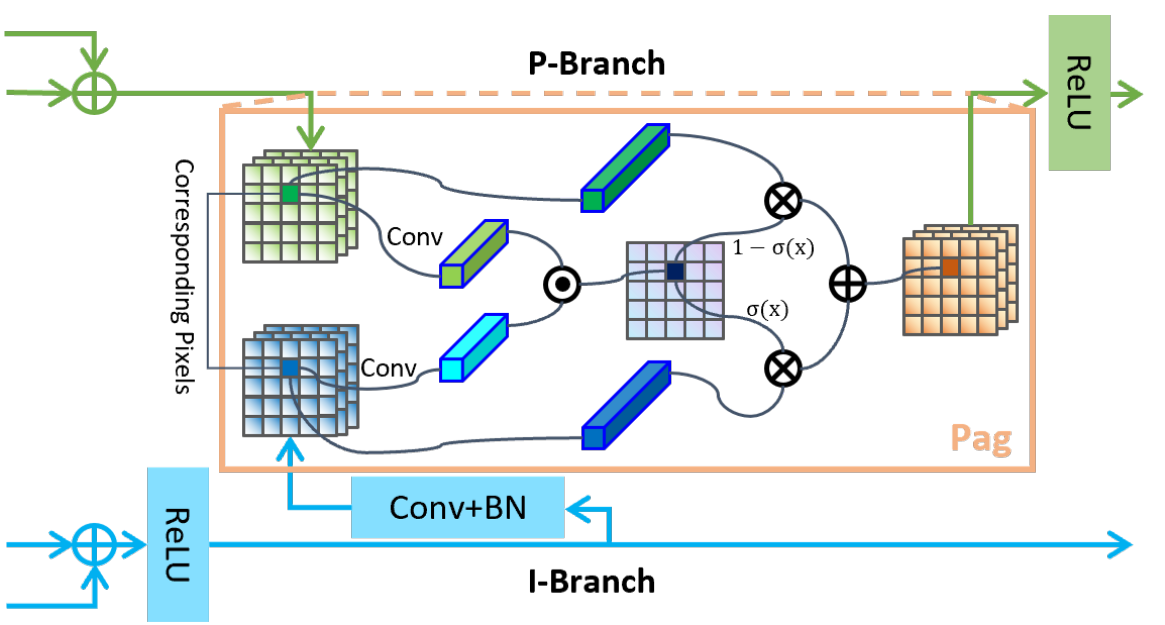
\includegraphics[width=.80\linewidth]{assets/pidnet/pag.png}
\caption{Pag dùng tương đồng giữa đặc trưng P và I để điều chỉnh lateral fusion. Trích Hình~5 của Xu và cộng sự \cite{pidnet}.}
\label{fig:paper-pag}
\end{figure}

\subsection{PAPPM: tổng hợp ngữ cảnh với độ trễ thấp}
Sau khi giảm độ phân giải, I cần ghép thông tin từ nhiều vùng quan sát. Pooling ở vùng nhỏ giữ ngữ cảnh lân cận; pooling trên toàn feature map cho biết bối cảnh chung của ảnh. DAPPM ghép các mức này theo chuỗi, nên mức sau phải chờ kết quả mức trước. PAPPM tổ chức lại để các mức được xử lý song song hơn và giảm số kênh mỗi mức từ 128 xuống 96. PIDNet-S/M dùng PAPPM để giảm độ trễ; PIDNet-L dùng DAPPM với số kênh được điều chỉnh.

\subsection{Bag và Light-Bag: dùng biên để điều tiết fusion}
Ở bước fusion cuối, thông tin biên giúp chọn giữa chi tiết và ngữ cảnh. Bag thực hiện phép chọn mềm theo công thức (9)--(10) của bài báo:
\begin{align}
 \boldsymbol\beta&=\operatorname{sigmoid}(\mathbf d),\label{eq:bag-attention}\\
 \mathbf y_{\mathrm{Bag}}&=f_{\mathrm{out}}\!\left(
 (1-\boldsymbol\beta)\odot\mathbf i+\boldsymbol\beta\odot\mathbf p\right).
 \label{eq:bag-fusion}
\end{align}
Trong đó, $\mathbf d$ là đặc trưng của D, $\boldsymbol\beta$ là hệ số sau sigmoid và $\odot$ là phép nhân theo phần tử. Phép $f_{\mathrm{out}}$ gồm convolution, BatchNorm và ReLU. Khi $\boldsymbol\beta$ lớn, Bag giữ nhiều đặc trưng P; khi nhỏ, Bag dùng nhiều đặc trưng I. Ở mép người đi bộ, P giúp giữ đúng đường viền. Trong vùng mặt đường rộng, I giúp dự đoán nhãn ổn định hơn. Hệ số này được tính cho từng kênh từ đặc trưng D; boundary head riêng mới tạo một điểm biên tại mỗi pixel.

\begin{figure}[htbp]
\centering
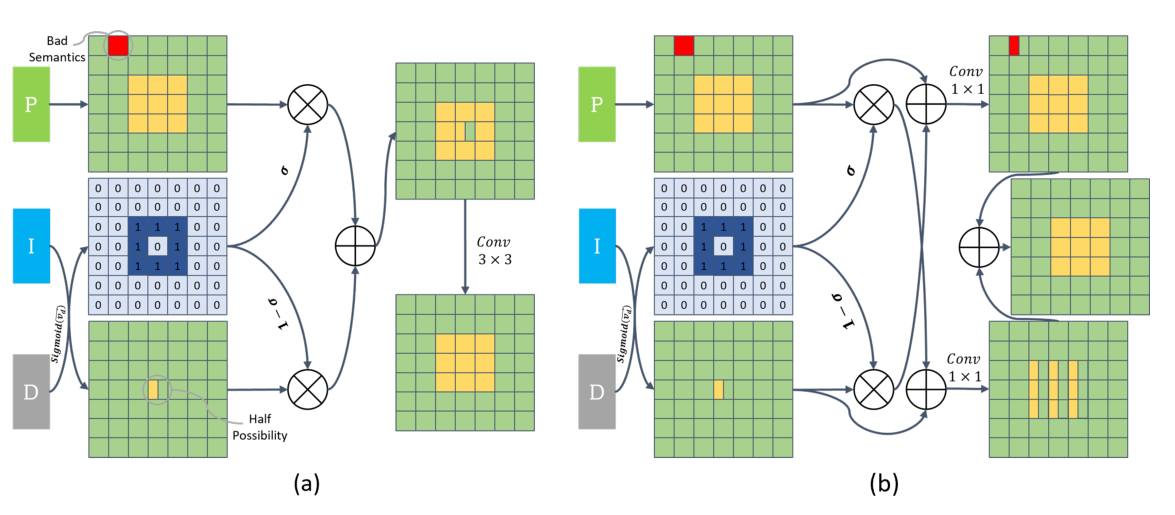
\includegraphics[width=.95\linewidth]{assets/pidnet/bag.png}
\caption{Bag (trái) và Light-Bag (phải) kết hợp P và I bằng tín hiệu D. Các ô màu minh họa vùng bên trong vật thể và vùng biên. Trích Hình~7 của Xu và cộng sự \cite{pidnet}.}
\label{fig:paper-bag}
\end{figure}

Light-Bag thay convolution $3\times3$ bằng hai luồng convolution $1\times1$, với công thức (11):
\begin{equation}
 \begin{split}
 \mathbf y_{\mathrm{Light}}={}&f_p\!\left((1-\boldsymbol\beta)\odot\mathbf i+\mathbf p\right)\\
                            &+f_i\!\left(\boldsymbol\beta\odot\mathbf p+\mathbf i\right).
 \end{split}
 \label{eq:light-bag}
\end{equation}
Ở đây, $f_p$ và $f_i$ là hai phép biến đổi convolution $1\times1$ kèm BatchNorm. Luồng thứ nhất giữ trực tiếp P và nhận thêm $(1-\boldsymbol\beta)\odot\mathbf i$; luồng thứ hai giữ trực tiếp I và nhận thêm $\boldsymbol\beta\odot\mathbf p$. Hai kết quả được cộng lại. Light-Bag nhờ đó vẫn dùng D để điều chỉnh trao đổi detail--context, với convolution nhẹ hơn Bag.

\section{Boundary supervision và hàm mục tiêu}
PIDNet phối hợp bốn loss:
\begin{equation}
 L_{\mathrm{PIDNet}}=0{,}4\ell_0+20\ell_1+\ell_2+\ell_3.
 \label{eq:pidnet-loss}
\end{equation}
Trong công thức (6), $\ell_0$ là auxiliary semantic cross-entropy sau Pag đầu tiên, giúp P học phân loại ngay ở tầng trung gian. $\ell_1$ là weighted boundary BCE, dùng trọng số để cân bằng nhóm pixel biên ít hơn nhóm không biên. $\ell_2$ là semantic cross-entropy ở đầu ra chính. $\ell_3$ là boundary-awareness cross-entropy, gọi tắt là BAS-Loss, tập trung vào lỗi phân loại tại những vị trí được dự đoán là biên. Nhãn cho boundary head được tạo từ mặt nạ phân đoạn bằng Canny rồi dilation.

BAS-Loss được viết trong công thức (5) của bài báo như sau:
\begin{equation}
 \ell_3=-\sum_{i,c}\mathbf{1}[b_i>0{,}8]\,
                   s_{i,c}\log\hat s_{i,c}.
 \label{eq:bas-loss}
\end{equation}
Ở đây, $b_i$ là điểm sigmoid của boundary head tại pixel $i$; $s_{i,c}$ bằng 1 nếu nhãn đúng là lớp $c$ và bằng 0 ở các lớp còn lại; $\hat s_{i,c}$ là xác suất mạng dự đoán cho lớp đó. Hàm chỉ thị $\mathbf{1}[b_i>0{,}8]$ giữ pixel có điểm biên lớn hơn 0,8 và bỏ các pixel khác khỏi BAS-Loss. Ba cơ chế dùng biên có vai trò riêng: BCE dạy D tìm biên, BAS nhấn mạnh lỗi ngữ nghĩa ở vùng biên dự đoán, còn Bag dùng đặc trưng D để ghép P và I. Ngưỡng 0,8 chỉ dùng cho BAS; Bag dùng hệ số sigmoid liên tục.

Biên ngữ nghĩa là nơi nhãn lớp thay đổi, chẳng hạn từ người sang mặt đường. Một vạch sơn hay bóng đổ có thể tạo cạnh ảnh mạnh nhưng vẫn thuộc cùng lớp Road. Nếu D nhầm các cạnh này thành biên, cả fusion và vùng được BAS chọn đều có thể bị ảnh hưởng. Đây là điểm cần xem xét khi phân tích những trường hợp dự đoán sai.

\section{Thí nghiệm và mức đóng góp của paper}
\subsection{Giao thức và kết quả chính}
Bài báo đánh giá trên Cityscapes, CamVid và PASCAL Context, dùng mIoU để đo độ chính xác. Mạng được pretrained trên ImageNet trước khi học phân đoạn; riêng CamVid tiếp tục từ trọng số Cityscapes. Trên Cityscapes, lịch train gồm 484 epoch, thay đổi tỷ lệ ảnh trong $[0{,}5;2{,}0]$ và crop $1024\times1024$. Tác giả dùng cả train và validation để huấn luyện mô hình nộp test Cityscapes/CamVid. Tốc độ trong bảng được đo trên một RTX 3090, batch size 1, sau khi gộp BatchNorm vào convolution.

\begin{table}[htbp]
\centering\small
\begin{tabularx}{\linewidth}{@{}Xlrr@{}}
\toprule
Mô hình & Dataset / tập & mIoU (\%) & FPS\\
\midrule
PIDNet-S & Cityscapes test & 78,6 & 93,2\\
PIDNet-M & Cityscapes test & 80,1 & 39,8\\
PIDNet-L & Cityscapes test & 80,6 & 31,1\\
PIDNet-S & CamVid test & 80,1 & 153,7\\
PIDNet-L & PASCAL Context validation, 59 lớp & 51,9 & --\\
\bottomrule
\end{tabularx}
\caption{Kết quả công bố trong Bảng~5--7 của PIDNet \cite{pidnet}. CamVid dùng Cityscapes pretraining. PASCAL Context dùng multi-scale và flip inference.}
\label{tab:paper-main-results}
\end{table}

Bảng~\ref{tab:paper-main-results} cho thấy PIDNet-L đạt mIoU cao hơn S trên Cityscapes, nhưng tốc độ giảm từ 93,2 xuống 31,1 FPS. PIDNet-S vì vậy phù hợp hơn khi ưu tiên tốc độ, còn L dành thêm tính toán để tăng độ chính xác. Trên PASCAL Context, PIDNet-L đạt 51,9\% mIoU với 59 lớp, so với 54,0\% của HRNet-W48 trong cùng bảng của bài báo. Đóng góp chính của PIDNet là cân bằng tốc độ và độ chính xác cho real-time segmentation.

\subsection{Đóng góp từng thành phần qua ablation}
Ablation thay đổi một hoặc một nhóm thành phần để xem chúng đóng góp thế nào. Bảng~1 bổ sung đồng thời nhánh D phụ và Bag vào hai baseline. BiSeNet--ResNet18 tăng từ 75,4 lên 76,7\% mIoU; DDRNet-23 tăng từ 79,5 lên 80,0\%. Đổi lại, FPS lần lượt giảm từ 63,2 xuống 52,1 và từ 51,4 xuống 39,2. Phép so sánh này đo tác dụng chung của nhánh biên và fusion.

Bảng~3 khảo sát riêng fusion và context aggregation trên PIDNet-S. Khi giữ PAPPM và thay phép cộng bằng Light-Bag, mIoU tăng từ 78,4 lên 78,8\%, còn tốc độ giảm từ 97,8 xuống 93,2 FPS. Khi giữ Light-Bag và thay DAPPM bằng PAPPM, mIoU vẫn là 78,8\% nhưng tốc độ tăng từ 83,7 lên 93,2 FPS. Như vậy, Light-Bag giúp tăng độ chính xác, còn PAPPM giảm thời gian xử lý trong các cặp đối chứng này.

Bảng~2 xem Pag và Bag có phối hợp hiệu quả hay không trên PIDNet-L pretrained. Dùng cả hai đạt 80,9\% mIoU, so với 80,7\% khi chỉ dùng phép cộng ở các kết nối và fusion. Hai cấu hình chỉ dùng một trong hai mô-đun đều đạt 80,5\%. Trong thí nghiệm này, kết hợp Pag với Bag tốt hơn thay riêng một thành phần.

Bảng~4 khảo sát cách giám sát trên PIDNet-L. Khi lần lượt thêm auxiliary semantic loss, boundary loss, BAS-Loss rồi OHEM, mIoU đi từ 78,6 qua 78,8; 79,9; 80,5 đến 80,9\%. Boundary loss tạo mức tăng 1,1 điểm phần trăm tại bước được thêm vào. BAS tiếp tục tăng 0,6 điểm phần trăm. OHEM (Online Hard Example Mining) ưu tiên các pixel mà mạng còn khó phân loại và tăng thêm 0,4 điểm phần trăm. Chuỗi này cho thấy cách tính loss đóng góp bên cạnh kiến trúc ba nhánh; mỗi mức tăng ứng với cấu hình ở ngay bước trước.

\section{Liên hệ với thiết kế thực nghiệm A2}
Thực nghiệm A2 chọn PIDNet-S trên CamVid và so sánh PIDNet-S đủ loss với PIDNet-S bỏ BAS-Loss. Bản đủ loss dùng bốn thành phần trong công thức~\eqref{eq:pidnet-loss}; bản bỏ BAS-Loss chỉ bỏ $\ell_3$, tức phần cross-entropy ngữ nghĩa bổ sung tại các pixel được dự đoán là biên. Cả hai giữ ba nhánh P/I/D, Pag, PAPPM, Light-Bag và các đầu dự đoán. Auxiliary semantic loss, weighted boundary BCE và main semantic loss với OHEM vẫn được tính ở cả hai.

Lựa chọn này xuất phát từ Bảng~4: sau khi đã học phân đoạn và biên, BAS tăng thêm giám sát ngữ nghĩa tại các pixel có điểm biên cao. A2 kiểm tra tác dụng đó trên PIDNet-S và CamVid, với cùng OHEM ở hai biến thể. Câu hỏi thực nghiệm là: việc nhấn mạnh thêm lỗi ở vùng biên dự đoán có cải thiện mIoU và IoU từng lớp hay không?
